\section{The Data-Capturing Process}
\label{sec:dataset:process}

Now that we have defined \textit{what} to mark up, we now describe the process to define \textit{how} we capture it. To do this, we need to first consider a way to encode both the  \textit{description} and \textit{constraints} of the data we wish to capture from within our dataset. The following sections refer to \textit{Argus} as a generic labelling tool, rather than its concrete implementation referred to in Section~\ref{sec:dataset:argus}.

This can be done in a four-step process: (1) informing Argus about what it is that we want to capture; (2) extracting information from our dataset; (3) transforming the data into an encodable format; and, (4) loading the data into an \gls{ai} model. Thus, the following sections describes the data capturing process as an informed \gls{etl} process. 

\subsection{Informing Argus}
\label{sec:dataset:process:informing}

Let us consider that the data we capture from Section~\ref{sec:dataset:architecture} can be placed into a structured hierarchical data format, represented using our metamodel. For convenience, we will refer to this hypothetical format as the \gls{adf}. Let's also assume that we can restrict the kind of data we want to capture using a set of constraint rules, which can be encoded into a hypothetical \gls{acl}. This, also, can be represented by our metamodel.

The first step is to feed in the constrains into a data capturer that restricts what kind of data we wish to read from our image dataset. This declarative format informs the capturer of the potential features, annotations and construction rules that is marked up by the annotator. For example, a concrete implementation of an \gls{acl} in an \glsac{xml} schema is given in Listing~\ref{lst:dataset:process:acl_sample}, where we define the features, annotations, conditions and dependencies of the image-level and $Bib$ segment-level features, using ID referencing inspired by \glsac{html}.

\clearpage

\begin{lstlisting}[language=ACL, label=lst:dataset:process:acl_sample, caption={[Sample Argus Constraint Language File Format] A hypothetical \glsx{acl} file describing the image-level and $BibSheet$ segment-level features as represented in an \gls{xml} schema.}]
<?xml version="1.0" encoding="utf-8"?>
<capture>
  <!-- Define the Image-Level Features -->
  <feature level="image" id="image">
    <annotation id="photo-crowded" type="boolean">
    </annotation>
    <annotation id="runners" type="collection">
      <!-- Condition that photo crowded is false -->
      <condition context="photo-crowded" value="self == false" />
    </annotation>
  </feature>
  
  <!-- Define the Bib Segment-Level Feature -->
  <feature level="segment" id="bib" owner="runners">
    <annotation id="bib-sheet" type="polygon">
      <!-- Condition that vertices must be 4 -->
      <condition context="bib-sheet" value="self.vertices == 4" />
    </annotation>
    <annotation id="rbn" type="label">
      <!-- Dependent on bib sheet to exist -->
      <dependency on="bib-sheet" />
    </annotation>
  </feature>
</capture>
\end{lstlisting}

Argus is therefore told what it is that it needs to capture, and---by using this declarative language---a \gls{ui} can automatically be generated to indicate to the marker the flow by which we must mark up information. 

\subsection{Extracting Features}
\label{sec:dataset:process:extracting}

Raw images are loaded into an `Annotate' mode of Argus, whereby the user interface is generated using the constraints discussed in Section~\ref{sec:dataset:process:informing}. Additionally, errors are now automatically shown when conditions or restrictions are not met. Each of the specific features can now be extracted using a number of the elements within the generated \gls{ui} as per those shown in Table~\ref{tab:dataset:process:ui_elements}, whereby the annotator follows the required steps (i.e., in dependency order) to carry out annotations. This, therefore, becomes the workflow of extraction which the annotator runs through---a concrete example of such a workflow for our case is shown in Figure~\ref{fig:dataset:process:argus_workflow}, as represented as a \gls{uml} activity diagram.

\begin{table}
  \centering
  \caption[Sample UI elements to extract features in Argus]{Sample \gls{ui} elements that can be made to extract features.}
  \label{tab:dataset:process:ui_elements}
    \begin{tabular}{lp{0.25\textwidth}p{0.5\textwidth}}
    \toprule
      \bfseries Annotation Type &
      \bfseries \gls{ui} Element(s) &
      \bfseries Usage
    \\
    \midrule
      Boolean &
      Checkbox &
      Check to indicate \textsc{true} value, \textsc{false} otherwise.
    \\
      Category &
      { Dropdown-Box \par Radio Button Group } &
      All variant Possible Values are shown as distinct options within a dropdown box's list items or as separate radio buttons.
    \\
      Label &
      Text Box &
      Text box shown to enter in label value.
    \\
      Colour &
      { Eye-Dropper \par Colour Wheel \par Colour Palette } &
      Selection of colour can be made from eye dropping a distinct colour in the image, from a selection of all colours in the colour wheel, or from a set of colours from a set colour palette.
    \\
      Polygon &
      Clicking $n_{vertices}$ times &
      Boundary is selected by clicking the required number of vertices around the selection area.
    \\
      Rectangle &
      Drag-And-Drop &
      A drag-and-drop around the required boundary is made.
    \\
    \bottomrule
    \end{tabular}
\end{table}

Additionally, the \gls{ui} elements can provide guidance to the tagger in the form of an instruction. For instance, annotations of a boolean type can be asked as a question: ``Is this photo crowded?''. Polygons can be specifically guided: ``Left click four times around the bib sheet region''. Similarly, the same can be done with a colour selection using an eye-dropper: ``Click the shorts of the runner to select their shorts colour''. These labels and \gls{ui} elements can be automatically generated based on the information supplied in the \glsx{acl} file.

Keyboard shortcuts can be automatically implemented to improve keyboard-driven navigation, reducing the need to use a mouse and automating responses (i.e., enter `Y' for `Yes' and `N' for `No')---ultimately to speed up the progression by which taggers extract these features.

Lastly, annotators can mark the image as `complete', indicating they are finished with all possible annotations in the dataset. This then produces an \glsx{adf} based on the image (Section~\ref{sec:dataset:process:transformation}). Once all images in the dataset are fully `complete', Argus informs that the extraction process on the entire dataset is now complete.

\begin{landscape}
\begin{figure}[p]
  \centering
  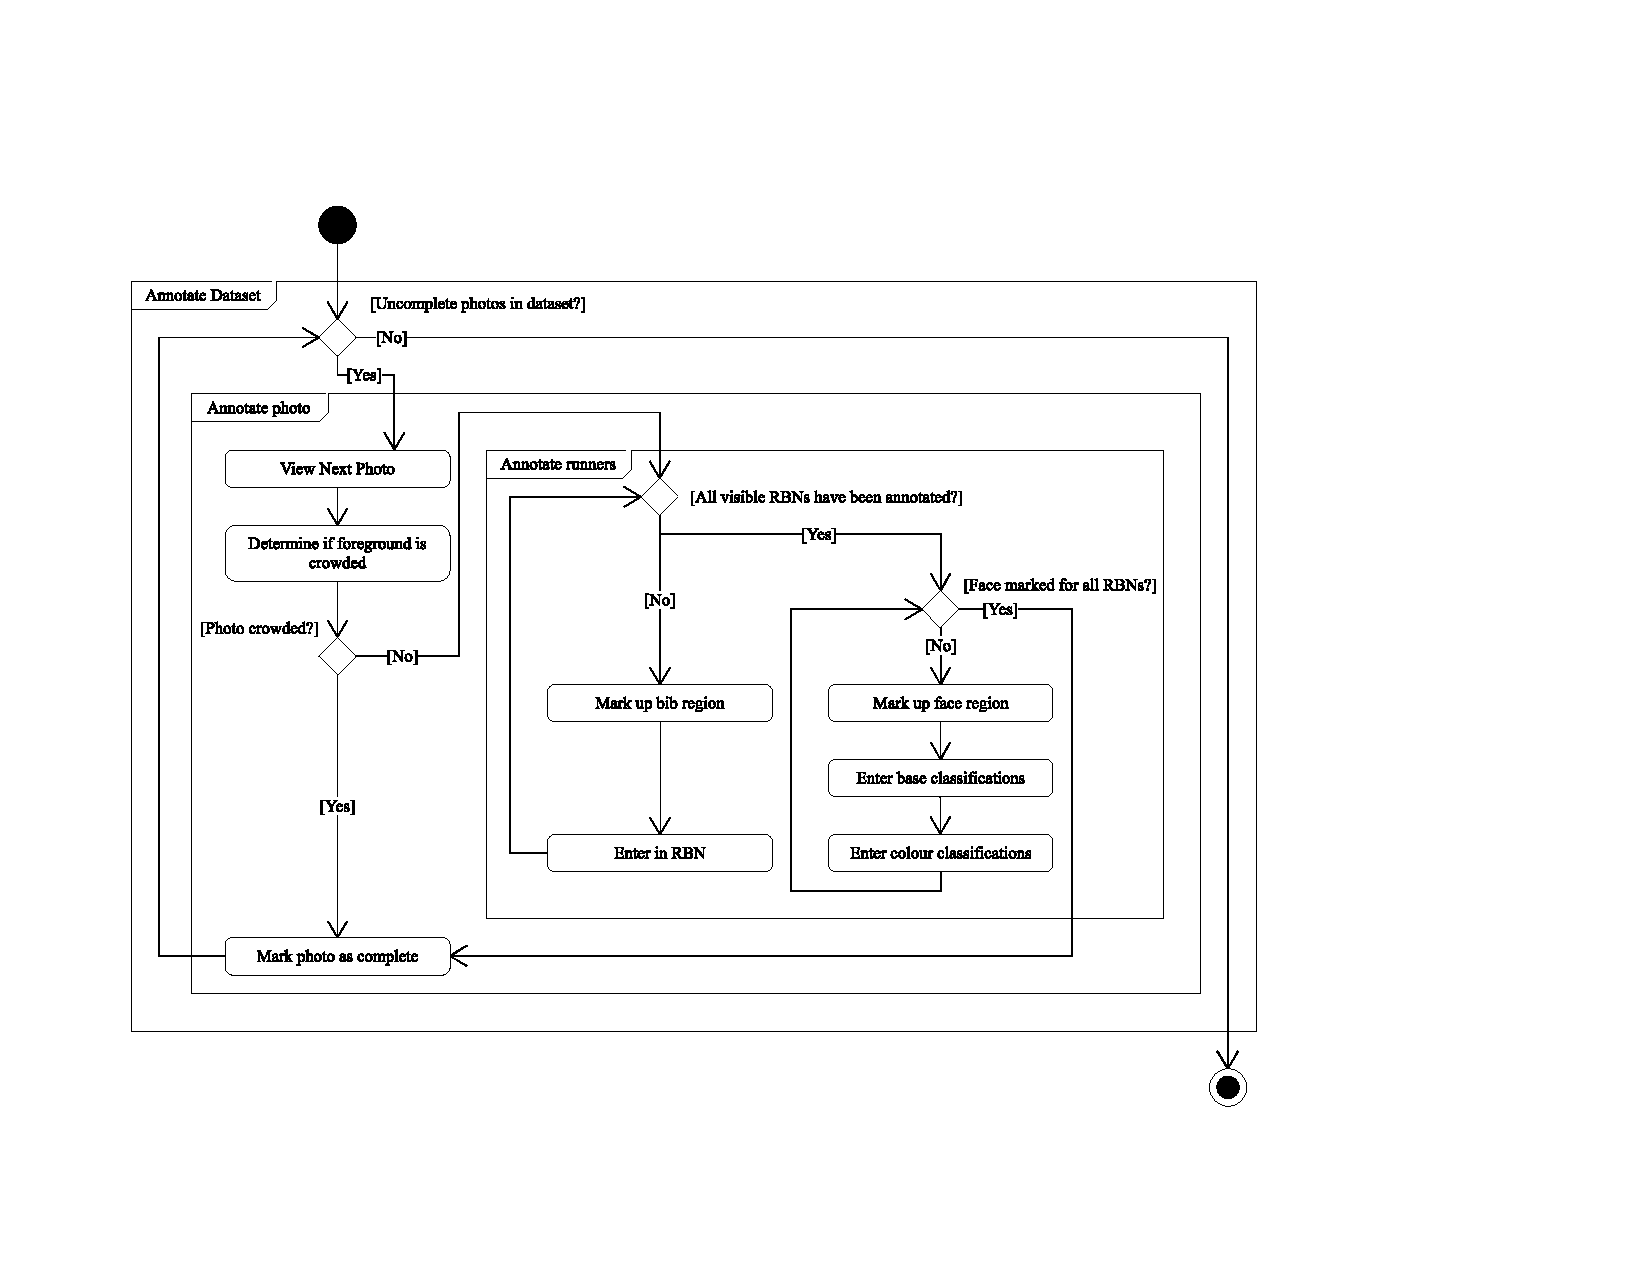
\includegraphics[width=0.9\paperwidth]{images/dataset/concrete_workflow}
  \caption[Concrete workflow example using Argus]{Concrete workflow of Argus in our bib annotation context. The \gls{acl} structures this process by defining dependency ordering.}
  \label{fig:dataset:process:argus_workflow}
\end{figure}
\end{landscape}

\subsection{Transformation}
\label{sec:dataset:process:transformation}

The features, once extracted, are automatically encoded into an \glsx{adf} upon marking the image as complete. To prevent data loss, files are encoded as the annotator progresses onto the next feature within the workflow of exatraction. All implicit attributes can be calculated given the explicit attributes manually entered by the runner at this stage.

A sample of an \gls{adf} in a language-agnostic tree format is shown in Figure~\ref{fig:dataset:adf_representation} for a photo with one runner. This could be serialised into any human-readable hierarchical format, such as a \glsac{yaml}, \glsac{json} or \gls{xml} file. Additionally, workflows from the \gls{acl} input file may be generated by a \gls{uml} activity diagram (as we have done in Figure~\ref{fig:dataset:process:argus_workflow}) to assist annotators in understanding how to mark up the photo. Thus, the transformation step \textit{universalises} the annotated data into a format readable by any supported parser of the \gls{adf} or \gls{acl} files. We propose examples of how this data is loaded in the following section.

\renewcommand*\DTstyle{\small\rmfamily}
\setlength{\DTbaselineskip}{15pt}

\begin{figure}
  \begin{subfigure}[b]{0.45\textwidth}
    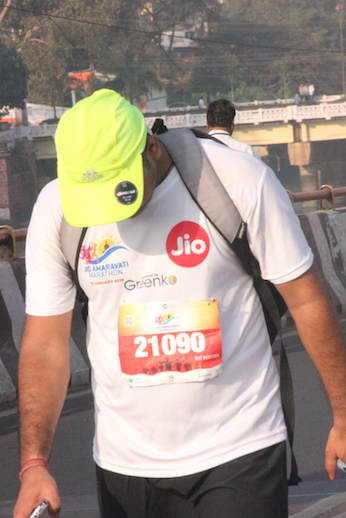
\includegraphics[width=\textwidth]{images/dataset/sample_annotated_runner}
  \end{subfigure}
  \vspace*{\fill}
  \hspace{-0.025\textwidth}
  \begin{subfigure}[b]{0.50\textwidth}
    \dirtree{%
      .1 \textbf{Image} \texttt{001}.  
      .2 PhotoCrowded : \textit{Boolean}.
      .3 \textsc{false}.
      .2 Runners : \textit{Collection}.
      .3 Runner \texttt{1}.
      .4 \textbf{Bib}.
      .5 Bounds : \textit{Polygon}.
      .6 $x_{1} = 1164, y_{1} = 2990$.
      .6 $x_{2} = 2147, y_{2} = 2990$.
      .6 $x_{3} = 2229, y_{3} = 3745$.
      .6 $x_{4} = 1215, y_{4} = 3807$.
      .5 RBN : \textit{Label}. 
      .6 \texttt{21090}.
      .4 \textbf{Face}.
      .5 Bounds : \textit{Rectangle}.    
      .6 $x_{1} = 512, y_{1} = 1034$.
      .6 $x_{2} = 1671, y_{2} = 2162$.
      .5 Gender : \textit{Category}.
      .6 \textsc{male}.
      .5 WearingHat : \textit{Boolean}.
      .6 \textsc{true}.
      .5 WearingGlasses : \textit{Boolean}.
      .6 \textsc{false}.
      .4 \textbf{Prominence}.
      .5 \gls{lop} : \textit{Category}.
      .6 \textsc{no}.
      .5 FaceVisible : \textit{Boolean}.
      .6 \textsc{false}.
      .5 Blurry : \textit{Boolean}.
      .6 \textsc{false}.
      .4 \textbf{Colours}.
      .5 ShirtColor : \textit{Color}.
      .6 $r = 255, g = 248, b = 239$.
      .5 ShoeColor : \textit{Color}.
      .6 $N/A$.
      .5 ShortsColor : \textit{Color}.
      .6 $r = 66, g = 63, b = 58$.
      .5 HatColor : \textit{Color}.
      .6 $r = 248, g = 255, b = 134$.
    }  
  \end{subfigure}
  \caption[Sample representation of an ADF]{Sample hierarchical data representation of an \gls{adf}, encoding the features (bolded) of the runner on the left. Implicit attributes are removed.}
  \label{fig:dataset:adf_representation}
\end{figure}

\subsection{Load}
\label{sec:dataset:process:load}

Once the data is transformed into a consistent format (i.e., an \gls{adf}), we are able to supply it to a number of different tools. In our research, we load the \gls{adf} into four tools:

\begin{enumerate}
  \item Argus is executed in `Review' mode, whereby a second annotator reviews the parsed annotations by loading a directory containing multiple \glspl{adf}. There they can run through a number checks to ensure the annotated data is accurate when training the \gls{ai} models.
  \item Custom augmenters load the \glspl{adf} as well as the source images to produce a number of variations on the image, essentially turning one image and its respective \gls{adf} into many variant images and \glspl{adf}. This is imperative when training our \gls{nn}, as explained in Section~\ref{sec:dataset:postprocessing:augmentation}.
  \item An adapter created for our \gls{nn} is used to load in an \gls{adf} and convert it into a \glsac{csv} of file paths to images, bounding boxes and labels. The \gls{nn} reads this file and uses it to learn where bib locations are in an image. This is later discussed in Chapter~\ref{ch:processing_pipeline}.
  \item We used Git\footnoteurl{https://git-scm.com}{11 Aug 2017} to track changes within our \gls{adf}. The benefit of serialising the data into a text file is that any version control management software can handle provenance for us (as suggested in Section~\ref{sec:dataset:architecture}), thereby sourcing changes in our \gls{ai} models easier by sourcing how the training data (i.e., \gls{adf} file) has derived over time.
\end{enumerate}

% GIT!



% Extract = Extract relevant features from the image
% Transform = Transform into ADF
% Load = Load by a human reviewer or into an AI or into a augmenter

% Talk about automatic mappings. e.g. drag and drop, \gls{ui} generation with descriptive labels etc. Things we can make the \gls{ui} automate
% Then discuss provenance and how we can track using git
